% !TEX root = ../main.tex

\section{Функції одного випадкового аргументу}
При розв'язанні задач іноді виникає необхідність визначити закон розподілу невипадкової функції від випадкового аргумента,
розподіл якого є відомим.
\subsection{Функції від дискретного випадкового аргументу}
Нехай $\xi$ --- дискретна випадкова величина з рядом розподілу 
\begin{center}
    \begin{tabular}{|c|c|c|c|c|c|}
        \hline
        $\xi$ & $x_1$ & $x_2$ & $...$ & $x_n$ & $...$ \\
        \hline
        $p$ & $p_1$ & $p_2$ & $...$ & $p_n$ & $...$ \\
        \hline
    \end{tabular}    
\end{center}
а $\varphi$ --- деяка вимірна числова функція, 
область визначення якої містить можливі значення $\xi$.
Можна розглядати випадкову величину $\eta = \varphi(\xi)$.

Очевидно, що $\eta$ --- теж ДВВ, що приймає значення $y_k = \varphi(x_k)$, 
$k = 1, 2, ...$ з ймовірностями $\P\{\eta = y_k\} = \P\{\xi = x_k : \varphi(x_k) = y_k\}$.
Якщо існує лише одне $\varphi^{-1} (y_k) = x_k$, то $\P\{\eta = y_k\} = \P\{\xi = x_k\} = p_k$.
Однак, можливо, що $y_k = \varphi(x_{k_1}) = \varphi(x_{k_2}) = ... = \varphi(x_{k_m})$.
Тоді $\P\{\eta = y_k\} = p_{k_1} + p_{k_2} + ... + p_{k_m}$.

\begin{example}
    Нехай $\xi$ має ряд розподілу
    \begin{center}
        \begin{tabular}{|c|c|c|c|c|c|}
            \hline
            $\xi$ & $-2$ & $-1$ & $0$ & $1$ & $2$ \\
            \hline
            $p$ & $1/9$ & $2/9$ & $1/9$ & $2/9$ & $3/9$ \\
            \hline
        \end{tabular}
    \end{center}
    Знайти закон розподілу $\eta = \xi^2$.
    
    З ряду розподілу $\xi$ видно, що $\xi^2$ приймає значення $0, 1, 4$ з
    ймовірностями $1/9$, $2/9 + 2/9$ та $1/9 + 3/9$.
    Отже, маємо ряд розподілу $\eta$: 
    \begin{center}
        \begin{tabular}{|c|c|c|c|}
            \hline
            $\eta$ & $0$ & $1$ & $4$ \\
            \hline
            $p$ & $1/9$ & $4/9$ & $4/9$ \\
            \hline
        \end{tabular}
    \end{center}
\end{example}

З побудови ряду розподілу функції від дискретного
випадкового аргументу випливає, що $\E(\varphi(\xi))^k = \sum\limits_{i=1}^{n(\infty)} \varphi^k(x_i) \P\{\xi = x_i\}$.

\subsection{Функції від неперервного випадкового аргументу}
Нехай $\xi$ --- неперервна випадкова величина, $f_\xi(x)$ --- її щільність розподілу, а $\varphi$ --- монотонна неперервна числова функція,
для якої обернена функція $\varphi^{-1}$ є диференційовною майже скрізь.
Розглянемо два випадки.

\begin{enumerate}
    \item $\eta = \varphi(\xi)$, де $\varphi$ --- монотонно зростаюча.

    \begin{tabular}{c p{8.8cm}}
        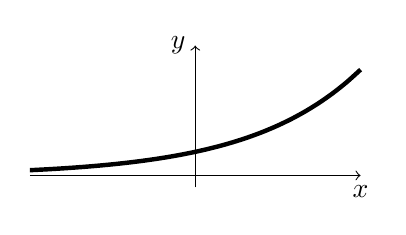
\begin{tikzpicture}[xscale = 0.7, yscale = 0.3, baseline={(current bounding box.north)}]
            \draw [->] (-3, 0) -- (3, 0);
            \draw [->] (0, -0.5) -- (0, 5.5);
            \draw [domain=-3:3, smooth, variable = \x, ultra thick] plot ({\x}, {e^(\x/2});
            \node [below] at (3, 0) {$x$};
            \node [left] at (0, 5.5) {$y$};
        \end{tikzpicture} &
        $F_\eta (y) = \P\left\{ \eta < y\right\} = \P\left\{ \varphi(\xi) < y\right\}$.

        Нехай $y = \varphi(x)$, тоді з монотонності $\varphi$ маємо рівність подій $\left\{ \varphi(\xi) < y\right\} = \left\{ \xi < x\right\}$.
        Тому $F_\eta (y) = F_\xi (x) = \int\limits_{-\infty}^x f_\xi(t) dt$. $\varphi$ має обернену, $x = \varphi^{-1} (y)$.
    \end{tabular}

    Отже, $F_\eta (y) = \int\limits_{-\infty}^{\varphi^{-1} (y)} f_\xi(t) dt$,
    $f_\eta(y) = F^\prime_\eta (y) = f_\xi\left(\varphi^{-1} (y)\right) \cdot \left(\varphi^{-1} (y) \right)^{\prime}$.
    \item $\eta = \varphi(\xi)$, де $\varphi$ --- монотонно спадна.
    
    \begin{tabular}{c p{8.8cm}}
        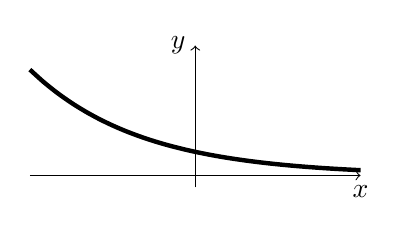
\begin{tikzpicture}[xscale = 0.7, yscale = 0.3, baseline={(current bounding box.north)}]
            \draw [->] (-3, 0) -- (3, 0);
            \draw [->] (0, -0.5) -- (0, 5.5);
            \draw [domain=-3:3, smooth, variable = \x, ultra thick] plot ({\x}, {e^(-\x/2});
            \node [below] at (3, 0) {$x$};
            \node [left] at (0, 5.5) {$y$};
        \end{tikzpicture} &
        $F_\eta (y) = \P\left\{ \eta < y\right\} = \P\left\{ \varphi(\xi) < y\right\}$.

        Нехай $y = \varphi(x)$, тоді з монотонності $\varphi$ маємо рівність подій $\left\{ \varphi(\xi) < y\right\} = \left\{ \xi > x\right\}$.
        Тому $F_\eta (y) = 1 - F_\xi (x) = 1 - \int\limits_{-\infty}^x f_\xi(t) dt$. $\varphi$ має обернену, $x = \varphi^{-1} (y)$.
    \end{tabular}

    Отже, $F_\eta (y) = 1 - \int\limits_{-\infty}^{\varphi^{-1} (y)} f_\xi(t) dt$,
    $f_\eta(y) = F^\prime_\eta (y) = - f_\xi\left(\varphi^{-1} (y)\right) \cdot \left(\varphi^{-1} (y) \right)^{\prime}$.
\end{enumerate}

\noindent Остаточно, для монотонної неперервної $\varphi$,
для якої обернена функція $\varphi^{-1}$ є диференційовною майже скрізь, має місце формула:
\begin{equation}\label{eq:phi_xi}
    \eta = \varphi(\xi), f_\eta(y) = f_\xi\left(\varphi^{-1} (y)\right) \cdot \left|\left(\varphi^{-1} (y) \right)^{\prime}\right|
\end{equation}
При цьому обов'язково треба зазначити допустимі значення $y$.

\begin{example}
    Нехай $\xi \sim \mathrm{U}(-\frac{\pi}{2}; \frac{\pi}{2})$. Знайти розподіл $\eta = \sin \xi$.

    \noindent $f_\xi(x) = \begin{cases}
        \frac{1}{\pi}, & |x| < \frac{\pi}{2} \\
        0, & |x| \geq \frac{\pi}{2}
    \end{cases}$, $\varphi(x) = \sin x$, $\varphi^{-1} (y) = \arcsin(y)$, $\left(\varphi^{-1} (y)\right)^{\prime} = \frac{1}{\sqrt{1-y^2}}$.
    $\eta$ може приймати значення від $-1$ до $1$. 
    Отже, $f_\eta(y) = \begin{cases}
        \frac{1}{\pi\sqrt{1-y^2}}, & |y| < 1 \\
        0, & |y| \geq 1
    \end{cases}$ --- це <<закон арксинуса>>.
\end{example}

\begin{example}
    Нехай $\xi \sim \mathrm{N}(a, \sigma^2)$. Знайти розподіл $\eta = e^\xi$.

    В цьому випадку $\varphi(x) = e^x$, $\varphi^{-1}(y) = \ln y$, $\left(\varphi^{-1} (y)\right)^{\prime} = \frac{1}{y}$.
    $\eta$ може приймати лише додатні значення, тому отримуємо щільність
    \begin{gather*}
        f_\eta(y) = \begin{cases}
            \frac{1}{\sqrt{2\pi}\sigma y} e^{-\frac{(\ln y-a)^2}{2\sigma^2}}, & y > 0 \\
            0, & y \leq 0
        \end{cases}
    \end{gather*}
    Розподіл $\eta$ називається \emph{логнормальним} (оскільки $\ln \eta$ має нормальний розподіл)
    та позначається $\eta \sim \mathrm{LogN}(a, \sigma^2)$.
\end{example}
\begin{exercise}
    Перевірити, що $\E\eta = e^{a + \frac{\sigma^2}{2}}$ і
    $\D\eta = \left(e^{\sigma^2} - 1\right) e^{2a + \sigma^2}$.
\end{exercise}

\begin{example}
    Нехай $\xi$ --- довільна НВВ, $F_\xi (x)$ --- її функція розподілу. 
    Знайти закон розподілу $\eta = F_\xi (\xi)$.

    \noindent $F_\eta (y) = \P\{\eta < y\} = \P\{F_\xi(\xi) < y\} = \P\{\xi < F_\xi^{-1}(y)\} = F_\xi(F_\xi^{-1}(y)) = \begin{cases}
        0, & y \leq 0 \\
        y, & 0 < y \leq 1 \\
        1, & y > 1
    \end{cases}$.

    \noindent Отже, $F_\xi (\xi) \sim U\left<0;1\right>$. Ще раз зауважимо, що результат має місце для довільної НВВ $\xi$.
\end{example}

\begin{remark}
    Якщо $\varphi$ не є неперервною, то $\eta = \varphi(\xi)$ може не бути НВВ. Наведемо декілька прикладів.
    \begin{enumerate}
        \item Нехай $\xi \sim \mathrm{Exp}(1)$. Знайдемо розподіл $\eta = \left[ \xi\right]$, де $\left[ \cdot\right]$ --- ціла частина.
        Оскільки ціла частина приймає значення $0, 1, 2, ...$, знайдемо відповідні ймовірності. 
        
        $\P\left\{ \left[ \xi\right] = n\right\} = \P\left\{ \xi \in [n; n+1)\right\} = \int\limits_n^{n+1} e^{-x} dx = e^{-n} - e^{-(n+1)} = e^{-n}(1 - e^{-1})$, $n = 0, 1, 2, ...$

        Отже, $\eta = \left[ \xi\right] \sim \mathrm{Geom}(1-e^{-1})$.

        За цим прикладом можна зробити висновок: якщо $\varphi$ --- кусково стала, а $\xi$ --- НВВ, то $\varphi(\xi)$ --- ДВВ.
        \item Нехай $\xi \sim \mathrm{Exp}(1)$. Знайдемо розподіл $\eta = \left\{ \xi\right\} = \xi - \left[ \xi\right]$. 
        В цьому випадку $\varphi$ є кусково неперервною функцією та приймає значення з інтервалу $[0; 1)$.
        
        Для $0< y < 1$ $F_\eta (y) = \P\left\{\eta < y\right\} = \P\left\{\eta \in [0; y)\right\} = \P\left\{\xi \in [n; n+y), n = 0, 1, 2, ...\right\}$.

        Для кожного $n$ $\P\left\{\xi \in [n; n+y)\right\} = \int\limits_n^{n+y} e^{-x} dx = e^{-n}(1 - e^{-y})$. 
        Отже, $\P\left\{\eta \in [0; y)\right\} = \sum\limits_{n=0}^{\infty} \P\left\{\xi \in [n; n+y)\right\} = (1 - e^{-y}) \sum\limits_{n=0}^{\infty} e^{-n} = \frac{1 - e^{-y}}{1 - e^{-1}}$. Отримали функцію розподілу $\eta$:

        $F_\eta (y) = \begin{cases}
            0, & y \leq 0 \\
            \frac{1 - e^{-y}}{1 - e^{-1}}, & 0 < y \leq 1 \\
            1, & y > 1
        \end{cases}$. Таким чином, $\eta$ --- НВВ.
    \end{enumerate}
\end{remark}

Узагальнимо формулу \eqref{eq:phi_xi} на випадок немонотонної функції $\varphi$.
Нехай $\xi$ --- НВВ, $f_\xi(x)$ --- її щільність розподілу, а $\varphi$ --- неперервна немонотонна числова функція.
Тоді область можливих значень $\xi$ можна розбити на проміжки, на яких $\varphi$ буде монотонною. 
Тоді, скориставшись результатом для монотонної функції, отримаємо формулу для щільності $\eta = \varphi(\xi)$:
\begin{equation}
    f_\eta (y) = \sum\limits_{k=1}^m f_\xi\left(\varphi_k^{-1} (y)\right) \cdot \left|\left(\varphi_k^{-1} (y) \right)^{\prime}\right|
\end{equation}
де $m$ --- кількість проміжків монотонності, а $\varphi_k^{-1}$ --- відповідні обернені функції, які мають бути диференційовними майже скрізь.

\begin{example}
    \begin{enumerate}
        \item $\xi \sim \mathrm{U}(-\frac{\pi}{2}, \frac{\pi}{2})$, знайти розподіл $\eta = \cos\xi$.

        На проміжках $(-\frac{\pi}{2}; 0]$ та $[0; \frac{\pi}{2})$ $\cos x$ є монотонною функцією, 
        відповідні обернені --- $\varphi_1^{-1} (y) = -\arccos y$, $\varphi_2^{-1} (y) = \arccos y$.

        Тоді $f_\eta (y) = \frac{1}{\pi} \cdot \left| - \frac{1}{\sqrt{1-y^2}}\right| + \frac{1}{\pi} \cdot \left|\frac{1}{\sqrt{1-y^2}}\right| = \begin{cases}
            \frac{2}{\pi} \frac{1}{\sqrt{1-y^2}}, & y \in [0; 1) \\
            0, & y \notin [0; 1)
        \end{cases}$.
        \item\label{ex:squared_norm_distr} $\xi \sim \mathrm{N}(a, \sigma)$, знайти розподіл $\eta = \xi^2$.

        На проміжках $(-\infty; 0]$ та $[0; +\infty)$ $x^2$ є монотонною функцією, 
        відповідні обернені --- $\varphi_1^{-1} (y) = -\sqrt{y}$, $\varphi_2^{-1} (y) = \sqrt{y}$.
        Щільність розподілу $\xi$ --- $f_\xi (x) = \frac{1}{\sqrt{2\pi}\sigma} e^{-\frac{(x-a)^2}{2\sigma^2}}$.

        Тоді $f_\eta (y) = \begin{cases}
            \frac{1}{\sqrt{2\pi}\sigma} e^{-\frac{(-\sqrt{y}-a)^2}{2\sigma^2}} \cdot \frac{1}{2\sqrt{y}} + 
        \frac{1}{\sqrt{2\pi}\sigma} e^{-\frac{(\sqrt{y}-a)^2}{2\sigma^2}} \cdot \frac{1}{2\sqrt{y}}, & y > 0 \\
        0, & y \leq 0
        \end{cases}$.

        При $\xi \sim \mathrm{N}(0, 1)$ $f_\eta(y) = \begin{cases}
            \frac{1}{\sqrt{2\pi y}} e^{-y/2}, y > 0 \\
            0, y \leq 0
        \end{cases}$, що означає $\xi^2 \sim \Gamma(\frac{1}{2}, \frac{1}{2})$.
    \end{enumerate}
\end{example}

\subsection{Числові характеристики функції неперервного випадкового аргументу}
Для функцій від ДВВ вже було отримано, що
$\E(\varphi(\xi))^k = \sum\limits_{i=1}^{n(\infty)} \varphi^k(x_i) \P\{\xi = x_i\}$.
Доведемо аналогічне твердження для функцій від НВВ.

\begin{proposition*}
    $\E (\varphi(\xi))^k = \int\limits_{-\infty}^{+\infty} \varphi^k(x) f_\xi(x) dx$ для всіх $k \in \mathbb{N}$.
\end{proposition*}
\begin{proof}
    Достатньо довести для монотонно зростаючої $\varphi$.

    \noindent$\eta = \varphi(\xi)$, $\E\eta^k = \int\limits_{-\infty}^{+\infty} y^k f_\eta(y) dy = \int\limits_{-\infty}^{+\infty} y^k f_\xi (\varphi^{-1} (y)) (\varphi^{-1} (y))^\prime dy =
    \int\limits_{-\infty}^{+\infty} y^k f_\xi(\varphi^{-1} (y)) d \varphi^{-1} (y) = \left[ \varphi^{-1} (y) = x, y = \varphi(x)\right] = \int\limits_{-\infty}^{+\infty} \varphi^k(x) f_\xi(x) dx$.
    У випадку монотонно спадної $\varphi$ під інтегралом отримаємо $-(\varphi^{-1} (y))^\prime$, а інтеграл після заміни змінної буде від $+\infty$ до $-\infty$.
    У випадку немонотонної $\varphi$ треба буде скористатися адитивністю інтеграла.
\end{proof}

\begin{remark}
    Для знаходження числових характеристик функції неперервного випадкового аргументу розподіл самої функції знаходити не потрібно.
\end{remark}

\begin{exercise}
    Дослідити, за яких умов на $\varphi$ ця формула має місце.
\end{exercise}

У випадках, коли $\varphi(x) = \cos (s x)$ або $\sin (s x)$ ($s\in \mathbb{R}$),
для знаходження числових характеристик можна скористатися характеристичною функцією $\xi$,
оскільки $\chi_{\xi}(s) = \E e^{i s \xi} = \E \cos(s\xi) + i \cdot\E\sin(s\xi)$,
тому $\E\cos(s\xi) = \mathrm{Re} \chi_{\xi}(s)$ і
$\E\sin(s\xi) = \mathrm{Im} \chi_{\xi}(s)$.
Для знаходження моментів вищих порядків можна скористатися формулами пониження степеня.